\section{Marching Triangles}
To create a mesh for an object we can use the simple Marching Triangles algorithm. The algorithm begins by creating a structured grid which completely contains the object. This structured grid is then split into triangles to form an unstructured grid. In this process we obtain a \textit{V} array containing the coordinates for the vertices and a \textit{T} array storing the connectivity of the triangles in the mesh. Each element in \textit{T} corresponds to a triangle, and thus \textit{T} is \textit{n} by 3 in size. Each of the three elements in a triangle encodes a vertex which when looked up in \textit{V} gives the coordinate to that vertex, and thus \textit{V} is \textit{m} by 2. The grid nodes are then assigned values depending on their distance to the object, thus creating a signed distance field. Without making any assumptions about our object, we will now most likely have several intersections between the grid lines and the object. What we are interested in now, is to find these intersections and recreate the mesh such that the triangles in our mesh match the borders of the object. When working in 2D we have eight possible cases which our triangles can 'be in'. The first scenario is all three vertices of a given triangle are outside the object. In this case we can simply remove the triangle from our mesh. The second case is all vertices in the triangle is inside the object in which case we just keep the triangle as it is. We then have three permutations where one vertex is outside the object but the other two vertices are inside. In this case we need to find the two intersection and interpolate the point outside onto the object towards the intersections. This results in a square which we will then have to split into two triangles. Lastly we have three permutations of having one point inside the object and two points outside. Here we again have to interpolate the outside vertices towards the intersections of the object. But in contrast to the previous case we get a new triangle here as we 'move' the two points outside the object onto the border of the object. To determine which case a triangle belongs to we look at the value of the signed distance to the object. If it is negative we are inside the object and if it is positive we are outside. We use the formula $sign(\phi(v1)) + sign(\phi(v2))\cdot2 + sign(\phi(v3))\cdot 4$ to determine which of the eight cases we are in. One should look at this like it being a bit mask where we find the sign of each vertex in a triangle. Vertex 1 is then responsible for the smallest bit, vertex 2 for the middle bit and vertex 3 for the last bit. This gives a unique mapping to the eight cases and we know exactly which vertices are inside and which are outside.\\
As we now know which vertices are inside the object and which are not, and we know what to do with these vertices, we now only missing how to find the intersections of the object and the grid lines. This can be done is several ways. One way, and the way I have implemented is the following. We use the mapping system described above to identify a triangle which has one or two vertices outside the object. We then create a vector from a point inside to a point outside. We then get the signed distance for the point inside to the object and the distance of the vector we created. We then create a ratio between these two distances and multiply this ratio with the vector we created. The idea being this ratio tells us how long we need to travel along the vector to get to the intersection. Moving a copy of our point inside along this our vector with the specified length we get closer to the intersection point. But as the signed distance we compute is likely shorter than diagonally distance we need to travel we repeat this process in a loop with the copied point. When we have iterated a few times we end up fairly close to the intersection point. This method has it shortcomings as very flat triangles would require a lot of iterations, and there are no guarantee the closest point of the object coincides with the vector we created and move along which means we might measure a wrong distance to move, however, this only measures too short a distance and so, in later iterations we will measure the distance to the correct border. The results using this approach to create a mesh can be seen in \autoref{ourmesh}.
\begin{figure}
	\centering
	\begin{subfigure}[b]{0.49\linewidth}
		\centering
		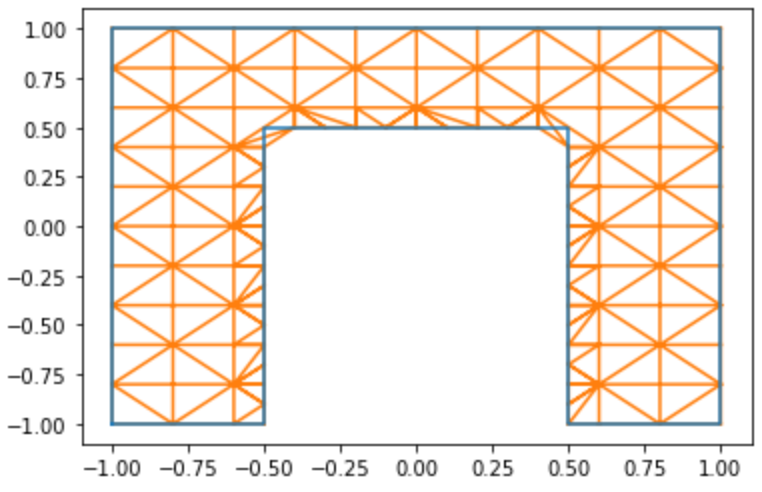
\includegraphics[width=\linewidth]{Materials/Triangles/mesh10}
		\caption{Triangle mesh generated with 10 by 10 nodes.}
	\end{subfigure}
	\hfill
	\begin{subfigure}[b]{0.49\linewidth}
		\centering
		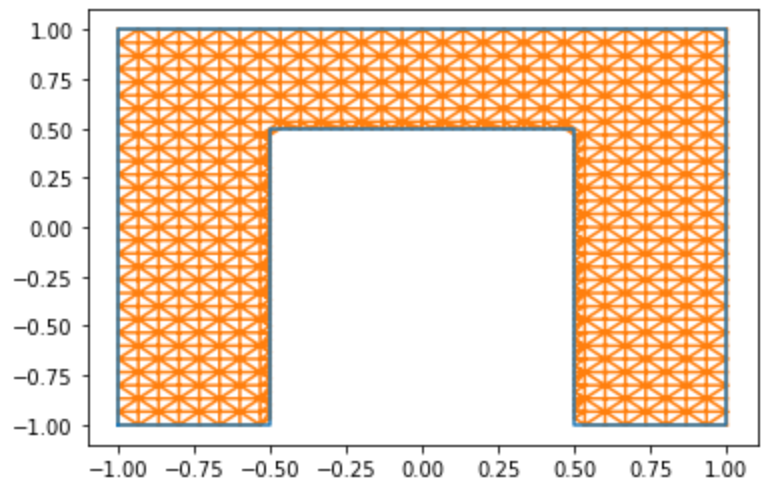
\includegraphics[width=\linewidth]{Materials/Triangles/mesh30}
		\caption{Triangle mesh generated with 30 by 30 nodes.}
	\end{subfigure}
	\caption{Two generated triangle meshes.}
	\label{ourmesh}
\end{figure} 
We see that the meshes are not perfect, lacking some triangles in some corners and 'taking too much corner' in others. These are unfortunately side effects of the Marching Triangles algorithm. Another perhaps simpler approach we could have used to find the intersections is a bisection. We here identify the two vertices which cross the border of our object and then find the midpoint between these two points. If the signed distance form the object to this midpoint is positive we are still outside and we can move the outside point to the midpoint. Otherwise we are inside and we can move the inside point to the midpoint. We can repeat this process in a loop until we are sufficiently close to the intersection.